\week{February 20, 1993}

\find{\paper{Alexander Vilenkin, Quantum cosmology, talk given at Texas/Pascos 1992 at Berkeley by available as \href{https://arxiv.org/abs/gr-qc/9302016}{arXiv:hep-th/9302016}.}}

This is, as Vilenkin notes, an elementary review of quantum cosmology. It won't be news to anyone who has kept up on that subject (except perhaps for a few speculations at the end), but for those who haven't been following this stuff, like myself, it might be a good way to get started.

Let's get warmed up....

Quantizing gravity is mighty hard. For one thing, there's the ``problem of time" - the lack of a distinguished time parameter in classical general relativity means that the usual recipe for quantizing a dynamical system - ``represent time evolution by the unitary operators $e^{-iHt}$ on the Hilbert space of states, where $t$ is the time and $H$, the Hamiltonian, is a self-adjoint operator" - breaks down! As Wheeler so picturesquely put it, in general relativity we have ``many-fingered time"; there are lots of ways of pushing a spacelike surface forwards in time.

But if we simplify the heck out of the problem, we might make a little progress. (This is a standard method in physics, and whether or not it's really justified, it's often the only thing one can do!) For one thing, note that in the big bang cosmology there is a distinguished ``rest frame" (or more precisely, field of timelike vectors) given by the galaxies, if we discount their small random motions. In reality these are maybe not so small, and maybe not so random - such things as the ``Virgo flow" show this - but we're talking strictly theory here, okay? - so don't bother us with facts! So, if we imagine that things go the way the simplest big bang models predict, the galaxies just sit there like dots on a balloon that is being inflated, defining a notion of ``rest" at each point in spacetime. This gives a corresponding notion of time, since one can measure time using clocks that are at rest relative to the galaxies. Then, since we are pretending the universe is completely homogeneous and isotropic - and let's say it's a closed universe in the shape of a 3-sphere, to be specific - the metric is given by

\[dt^2 - r(t)^2[(d\psi)^2 + (sin\psi^2{(d\theta)^2 + (sin\theta^2 (d\varphi)^2}]\]

What does all this mean? Here r(t) is the radius of the universe as a function of time, the following stuff is just the usual metric on the unit 3-sphere with hyperspherical coordinates $\psi, \theta, \varphi$ generalizing the standard coordinates on the 2-sphere we all learn in college:

\[(d\psi)^2 + (\sin\psi )^2((d\theta)^2 + (\sin\theta)^2 (d\varphi)^2)\]

and the fact that the metric on spacetime is $dt^2$ minus a bunch of stuff reflects the fact that spacetime geometry is ``Lorentzian," just as in flat Minkowski space the metric is

\[dt^2 - dx^2 - dy^2 - dz^2\]

The name of the game in this simple sort of big bang cosmology is thus finding the function $r(t)$! To do this, of course, we need to see what Einstein's equations reduce to in this special case, and since Einstein's equations tell us how spacetime curves in response to the stress-energy tensor, this will depend on what sort of matter we have around. We are assuming that it's homogeneous and isotropic, whatever it is, so it turns out that all we need to know is its density $\rho$ and pressure $P$ (which are functions of time). We get the equations

$$\frac{r''}{r} = -(4\pi/3)(\rho + 3P) \quad \quad (r')^2 = (8\pi/3) \rho r^2 - 1$$

Here primes denote differentiation with respect to $t$, and I'm using units in which the gravitational constant and speed of light are equal to 1.

Let's simplify this even more. Let's assume our matter is ``dust," which is the technical term for zero pressure. We get two equations:
\begin{equation}\label{eq:1}
    \frac{r''}{r} = -(4\pi/3)\rho \quad \quad (r')^2 = (8\pi/3) \rho r^2 -1 
\end{equation}
Now let's take the second one, differentiate with respect to $t$,

\[2r''r' = (8\pi/3)(\rho'r^2 + 2\rho rr')\]

plug in what the first equation said about $r''$,

\[-(8\pi/3) \rho r r' = (8\pi/3)(\rho' r^2 + 2\rho r r')\]

clear out the crud, and lo:

\[3\rho r' = -\rho' r\]

or, more enlighteningly,

\[\frac{d(\rho r^3)}{dt} = 0\]

This is just ``conservation of dust" - the dust density times the volume of the universe is staying constant. This, by the way, is a special case of the fact that Einstein's equations automatically imply local conservation of energy (i.e., that the stress-energy tensor is divergence-free).

Okay, so let's say $\rho r^3 = D$, with $D$ being the total amount of dust. Then we can eliminate $\rho$ from \eqref{eq:1} and get:
\begin{equation}\label{eq:2}
    r'' = \frac{-4\pi D}{3r^2} \quad \quad (r')^2 - (8\pi/3) \frac{D}{r} = -1 
\end{equation}
What does this mean? Well, the first one looks like it's saying there's a force trying to make the universe collapse, and that the strength of this force is proportional to $1/r^2$. Sound vaguely familiar? It's actually misleadingly simple - if we had put in something besides dust it wouldn't work quite this way - but as long as we don't take it too seriously, we can just think of this as gravity trying to get the universe to collapse. And the second one looks like it's saying that the ``kinetic" energy proportional to $(r')^2$, plus the ``potential" energy proportional to $\frac{-1}{r}$, is constant! In other words, we have a nice analogy between the big bang cosmology and a very old-fashioned system, a classical particle in one dimension attracted to the origin by a $\frac{1}{r^2}$ force!

It's easy enough to solve this equation, and easier still to figure it out qualitatively. The key thing is that since the total ``energy" in the second equation of \eqref{eq:2} is negative, there won't be enough ``energy" for r to go to infinity, that is, there'll be a big bang and then a big crunch. Here's r as a function of t, roughly:

\begin{center}
  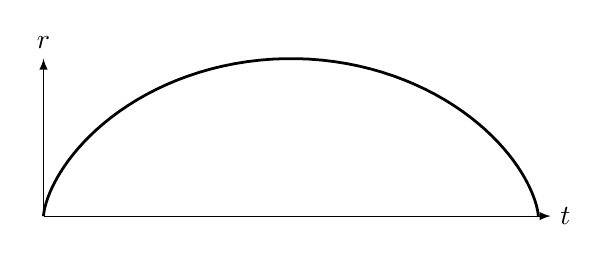
\begin{tikzpicture}
  \coordinate (O) at (0,0);
  \coordinate (A) at (0,2);
  \def\r{20} % radius
  \def\c{3} % center
  \coordinate (C) at (\c, \r);


  \draw[-latex] (O) -- (A) node[anchor=south] {$r$};
  \draw[-latex] (O) -- (2.05*pi,0) node[anchor=west] {$t$};
  \draw[black,domain=0:2*pi,samples=80, line width=1] 
       plot ({\x - sin(\x r)},{1 - cos(\x r)});
  \end{tikzpicture}
\end{center}
  
What goes up, must come down! This curve, which I haven't drawn too well, is just a cycloid, which is the curve traced out by a point on the rim of rolling wheel. So, succumbing to romanticism momentarily we could call this picture ONE TURN OF THE GREAT WHEEL OF TIME.... But there is no reason to expect further turns, because the differential equation simply becomes singular when $r = 0$. We may either say it doesn't make sense to speak of ``before the big bang" or ``after the big crunch" - or we can look for improved laws that avoid these singularities. (I should repeat that we are dealing with unrealistic models here, since for example there is no evidence that there is enough matter around to ``close the universe" and make this solution qualitatively valid - it may well be that there's a big bang but no big crunch. In this case, there's only one singularity to worry about, not two.)

People have certainly not been too ashamed to study the quantum theory of this system (and souped-up variants) in an effort to get a little insight into quantum gravity. We would expect that quantum effects wouldn't matter much until the radius of the universe is very small, but when it is very small they would matter a lot, and maybe - one might hope - they would save the day, preventing the nasty singularities. I'm not saying they DO - this is hotly debated - but certainly some people hope they do. Of course, serious quantum gravity should take into account the fact that geometry of spacetime has all sorts of wiggles in it -it isn't just a symmetrical sphere. This may make a vast difference in how things work out. (For example, the big crunch would be a lot more exciting if there were lots of black holes around by then.) The technical term for the space of all metrics on space is ``superspace" (sigh), and the toy models one gets by ignoring all but finitely many degrees of freedom are called ``minisuperspace" models.

Let's look at a simple minisuperspace model. The simplest thing to try is to take the classical equations of motion \eqref{eq:2} and try to quantize them just like one would a particle in a potential. This is a delicate business, by the way, because one can't just take some classical equations of motion and quantize them in any routine way. There are lots of methods of quantization, but all of them require a certain amount of case-by-case finesse.

The idea of ``canonical quantization" of a classical system with one degree of freedom - like our big bang model above, where the one degree of freedom is $r$ - is to turn the ``position" (that's $r$) into a multiplication operator and the ``momentum" (often that's something like $r'$, but watch out!) into a differentiation operator, say $-i\hbar \frac{d}{dr}$, so that we get the ``canonical commutation relations"
\[[-i\hbar \frac{d}{dr},r] = -i\hbar\]
We then take the formula for the energy, or Hamiltonian, in terms of position and momentum, and plug in these operators, so that the Hamiltonian becomes an operator. (Here various ``operator-ordering" problems can arise, because the position and momentum commuted in the original classical system but not anymore!) To explain what I mean, why don't I just do it!

So: I said that the formula
\begin{equation}
    (r')^2 - (8\pi/3) \frac{D}{r} = -1
\end{equation}
looks a lot like a formula of the form ``kinetic energy plus potential energy is constant". Of course, we could multiply the whole equation by anything and get a valid equation, so it's not obvious that the ``right'' Hamiltonian is
\[(r')^2 - (8\pi/3) \frac{D}{r}\]
or (adding 1 doesn't hurt)
\[(r')^2 - (8\pi/3) \frac{D}{r} + 1\]

In fact, note that multiplying the Hamiltonian by some function of $r$ just amounts to reparametrizing time, which is perfectly fine in general relativity. In fact, Vilenkin and others before him have decided it's better to multiply the Hamiltonian above by $r^2$. Why? Well, it has to do with figuring out what the right notion of ``momentum" is corresponding to the ``position" $r$. Let's do that. We use the old formula
\[p = \frac{dL}{dq'}\]

relating momentum to the Lagrangian, where for us the position, usually called $q$, is really $r$.

The Lagrangian of general relativity is the ``Ricci scalar" $R$ - a measure of curvature of the metric - and in the present problem it turns out to be
\[R = 6(\frac{r''}{r} + \frac{(r')^2}{r^2})\]
But we are reducing the full field theory problem down to a problem with one degree of freedom, so our Lagrangian should be the above integrated over the 3-sphere, which has volume \[16\pi\frac{r^3}{3}\] giving us \[32\pi (r''r^2 + (r')^2 r)\]

However, the $r''$ is a nuisance, and we only use the integral of the Lagrangian with respect to time (that's the action, which classically is extremized to get the equations of motion), so let's do an integration by parts, or in other words add a total divergence, to get the Lagrangian

Differentiating with respect to $r'$ we get the momentum ``conjugate to $r$", \[p = -64\pi r'r\]
Now I notice that Vilenkin uses as the momentum simply $-r'r$, somehow sweeping the monstrous $64\pi$ under the rug. I have the feeling that this amounts to pushing this factor into the definition of $\hbar$ in the canonical commutation relations. Since I was going to set $\hbar$ to 1 in a minute anyway, this is okay (honest). So let's keep life simple and use
\[p = r'r\]
Okay! Now here's the point, we want to exploit the analogy with good old quantum mechanics, which typically has Hamiltonians containing something like $p^2$. So let's take our preliminary Hamiltonian
\[(r')^2 -(8\pi/3) \frac{D}{r} + 1\]
and multiply it by $r^2$, getting
\[H = p^2 - (8\pi \frac{D}{3})r + r^2\].
Hey, what's this? A harmonic oscillator! (Slightly shifted by the term proportional to $r$.) So the universe is just a harmonic oscillator... I guess that's why they stressed that so much in all my classes!

Actually, despite the fact that we are working with a very simple model of quantum cosmology, it's not quite that simple. First of all, recall our original classical equation, \eqref{eq:3}. This constrained the energy to have a certain value. I.e., we are dealing not with a Hamiltonian in the ordinary sense, but a ``Hamiltonian constraint" - typical of systems with time reparametrization invariance. So our quantized equation says that the ``wavefunction of the universe," $\Psi(r)$, must satisfy
\[H\Psi = 0\]
Also, unlike the ordinary harmonic oscillator we have the requirement that $r > 0$. In other words, we're working with a problem that's like a harmonic oscillator and a ``wall" that keeps $r > 0$. Think of a particle in a potential like this:
%FIGURE THIS PLOT OUT
\begin{center}
  \begin{tikzpicture}
  \coordinate (O) at (0,0);
  \coordinate (A) at (0,2);
  \def\r{20} % radius
  \def\c{3} % center
  \coordinate (C) at (\c, \r);


  \draw[-latex] (O) -- (A) node[anchor=south] {$V(r)$};
  \draw[-latex] (O) -- (2.05*pi,0) node[anchor=west] {$r$};
  \draw[black,domain=0:2*pi,samples=80, line width=1] 
       plot ({\x^2 r});
  \end{tikzpicture}
\end{center}

Here $V(r) = - (8\pi \frac{D}{3})r + r^2$. The minimum of $V$ is at $r = 4\pi \frac{D}{3}$ and the zeroes are at $r = 0$ and $8\pi \frac{D}{3}$. Classically, a particle with zero energy starting at $r = 0$ will roll to the right and make it out to $r = 4\piD\frac{D}{3}$ before rolling back to $r = 0$. This is basically the picture we had in Figure 1, except that we've reparametrized time so we have simple harmonic motion instead of cycloid.
Quantum mechanically, however one must pick boundary conditions at $r = 0$ to make the problem well-defined!

This is where the fur begins to fly!! Hawking and Vilenkin have very different ideas about what the right boundary conditions are. And note that this is not a mere technical issue, since they determine the wavefunction of the universe in this approach! I will not discuss this since Vilenkin does so quite clearly, and if you understand what I have written above you'll be in a decent position to understand him. I will just note that Vilenkin, rather than working with a universe full of ``dust," considers a universe in which the dominant contribution to the stress-energy tensor is the cosmological constant, that is, the negative energy density of a ``false vacuum", which believers in inflation (such as Vilenkin) think powered the exponential growth of the universe at an early stage. So his equations are slightly different from those above (and are only meant to apply to the early history of the universe).

[Let me just interject a question to the experts if I may - since I've written this long article primarily to educate myself. It would seem to me that the equation $H\Psi = 0$ above would only have a normalizable solution if the boundary conditions were fine-tuned! I.e., maybe the equation $H\Psi = 0$ itself determines the boundary conditions! This would be very nice; has anyone thought of this? It seems reasonable because, with typical boundary conditions, the operator $H$ above will have pure point spectrum (only eigenvalues) and it would be rather special for one of them to be 0, allowing a normalizable solution of $H\Psi = 0$. Also, corrections and education of any sort are welcomed. I would love to discuss this with some experts.]

Anyway, suppose we find some boundary conditions and calculate $\Psi$, the ``wavefunction of the universe." (I like repeating that phrase because it sounds so momentous, despite the fact that we are working with a laughably oversimplified toy model.) What then? What are the implications for the man in the street?

Let me get quite vague at this point. Think of the radius of the universe as analogous to a particle moving in the potential of Figure 2. In the current state of affairs classical mechanics is an excellent approximation, so it seems to trace out a classical trajectory. Of course it is really obeying the laws of quantum mechanics, so the trajectory is really a ``wave packet" - technically, we use the WKB approximation to see how the wave packet can seem like a classical trajectory. But near the big bang or big crunch, quantum mechanics matters a lot: there the potential is rapidly varying (in our simple model it just becomes a ``wall") and the wave packet may smear out noticeably. (Think of how when you shoot an electron at a nucleus it bounces off in an unpredictable direction - it's wavefunction just tells you the probability that it'll go this way or that!) So some quantum cosmologists have suggested that if there is a big crunch, the universe will pop back out in a highly unpredictable, random kind of way!

I should note that Vilenkin has a very different picture. Since this stuff makes large numbers of assumptions with very little supporting evidence, it is science that's just on the brink of being mythology. Still, it's very interesting.
\find{\paper{Lee Smolin, Finite, diffeomorphism invariant observables in quantum gravity, available as \href{https://arxiv.org/abs/gr-qc/9302011}{gr-qc/9302011.}}}
The big problem in canonical quantization of gravity, once one gets beyond ``mini-" and ``minisuperspace" models, is to find enough diffeomorphism-invariant observables. There is a certain amount of argument about this stuff, and various approaches, but one common viewpoint is that the ``physical" observables, that is, the really observable observables, in general relativity are those that are invariant under all diffeomorphisms of spacetime. I.e., those that are independent of any choice of coordinates. For example, saying ``My position is (242,2361,12,-17)" is not diffeomorphism-invariant, but saying ``I'm having the time of my life" is. It's hard to find lots of (tractable) diffeomorphism invariant observables - or even any! Try figuring out how you would precisely describe the shape of a rock without introducing any coordinates, and you'll begin to see the problem. (The quantum mechanical aspects make it harder.)

Rovelli came up a while back with a very clever angle on this problem. It's rather artificial but still a big start. Using a ``field of clocks" he was able to come up with interesting diffeomorphism invariant observables. The idea is simply that if you had clocks all around you could say ``when the bells rang 2 a.m. I was having the time of my life" - and this would be a diffeomorphism-invariant statement, since rather than referring to an abstract coordinate system it expresses the coincidence of two physical occurences, just like ``the baseball broke through the window". Then he pushed this idea to define ``evolving constants of motion" - a deliberate oxymoron - to deal with the famous ``problem of time" in general relativity: how to treat time evolution in a coordinate-free manner on a spacetime that's not flat and, worse, whose geometry is ``uncertain" a la Heisenberg? This is treated, by the way, in

\find{\paper{Carlo Rovelli, Time in quantum gravity: an hypothesis, Phys. Rev. D43 (1991), 442-456.}}
Also, an excellent and very thorough review of the problem of time and various proposed solutions, including Rovelli's, is given in
\find{\paper{Chris J. Isham, Canonical quantum gravity and the problem of time, 125 pages, available as \href{https://arxiv.org/abs/gr-qc/9210011}{gr-qc/9210011.}}}

Anyway, in a paper I very briefly described in {\hyperref[week1]{week1.tex}}

\find{\paper{Lee Smolin, Time, measurement and information loss in quantum cosmology, available as \href{https://arxiv.org/abs/gr-qc/9301016}{gr-qc/9301016}}}

Smolin showed, how, using a clever trick sketched in the present paper to get ``observables" invariant under spatial but not temporal observables, together with Rovelli's idea, one could define lots of REAL observables, invariant under spacetime diffeomorphisms that is, thus making a serious bite into this problem.

I warn the reader that there is a fair amount that is not too realistic about these methods. First there's the ``clock field" - this can actually be taken as a free massless scalar field, but in so doing there is the likelihood of serious technical problems. Some of these are discussed in
\find{\paper{P. Hajicek, Comment on ``Time in quantum gravity - an hypothesis", Phys. Rev. D44 (1991), 1337-1338.}}
(But I haven't actually read this, just Isham's description.) Also, the clever trick of the present paper is to couple gravity to an antisymmetric tensor gauge field so that in addition to having loops as part of ones "loop representation," one has surfaces - a ``surface representation". But this antisymmetric tensor gauge field is not the sort of thing that actually seems to arise in physics (unless I'm missing something). Still, it's a start. I think I'll finish by quoting Smolin's abstract:
\begin{quote}
    Two sets of spatially diffeomorphism invariant operators are constructed in the loop representation formulation of quantum gravity. This is done by coupling general relativity to an anti- symmetric tensor gauge field and using that field to pick out sets of surfaces, with boundaries, in the spatial three manifold. The two sets of observables then measure the areas of these surfaces and the Wilson loops for the self-dual connection around their boundaries. The operators that represent these observables are finite and background independent when constructed through a proper regularization procedure. Furthermore, the spectra of the area operators are discrete so that the possible values that one can obtain by a measurement of the area of a physical surface in quantum gravity are valued in a discrete set that includes integral multiples of half the Planck area. These results make possible the construction of a correspondence between any three geometry whose curvature is small in Planck units and a diffeomorphism invariant state of the gravitational and matter fields. This correspondence relies on the approximation of the classical geometry by a piecewise flat Regge manifold, which is then put in correspondence with a diffeomorphism invariant state of the gravity-matter system in which the matter fields specify the faces of the triangulation and the gravitational field is in an eigenstate of the operators that measure their areas.
\end{quote}


